% Emerging Liability Severity Under Sparse Claims
% Self-contained LaTeX (no external .bib): compiles on Overleaf or with tectonic.
% Realistic target venue: Variance (CAS) or Risks (MDPI) — an APPLIED synthesis,
% not a theorem paper (the methods are recombinations of known results).
% Revised to remove overclaims and unsupported empirical assertions flagged by a
% four-persona review panel (actuary, AI architect, liability lawyer, editor).
\documentclass[11pt]{article}
\usepackage[margin=1in]{geometry}
\usepackage{amsmath,amssymb,amsthm}
\usepackage{booktabs}
\usepackage{natbib}
\usepackage{xcolor}
\usepackage{hyperref}
\usepackage{url}
\usepackage{graphicx}
\graphicspath{{figures/}{paper/figures/}}
\newtheorem{lemma}{Lemma}
\newtheorem{proposition}{Proposition}
\newtheorem{corollary}{Corollary}
\newtheorem{remark}{Remark}
\DeclareMathOperator{\Var}{Var}

\title{\textbf{Emerging Liability Severity Under Sparse Claims:\\
Disclosure Censoring and the Identifiability Frontier\\
with an Illustrative Application to AI Systems}}
\author{Tayyub Yaqoob\\\small Independent Researcher}
\date{Working draft --- \today}

\begin{document}
\maketitle

\begin{abstract}
\noindent
Pricing emerging liability risks before a mature claims history exists is a recurring
actuarial problem, from catastrophe modelling to cyber. Public incident data for such risks
are sparse and \emph{disclosure-censored}: only losses above an effective reporting threshold
enter the public record, so a severity estimate must borrow strength from mature proxy lines.
We frame the question as one of \emph{identifiability}: borrowing from a proxy through a
commensurate prior, \emph{when does a data-poor line's severity posterior transition from
prior-driven to data-driven?} We make three contributions. (i)~We argue that loss frequency is
structurally non-identifiable from public incident catalogues (no exposure denominator), so an
emerging-risk analysis is necessarily severity-first. (ii)~We define an \emph{identifiability
frontier} $n^\star$ at which the posterior escapes the prior, recover the classical
B\"uhlmann--Straub factor as its conjugate special case, and show that left-truncation deflates
the effective sample size by a factor $1-\delta(\alpha)$, inflating $n^\star$ by
$1/(1-\delta(\alpha))$ (Lemma~1, Corollary~1; numerically validated). (iii)~We illustrate the
lens on a public-record screen of AI-attributed losses. Our empirical contribution is
deliberately modest: we report a screening funnel and an \emph{illustrative} convenience set,
and show that the prior-driven-versus-data-driven verdict is \emph{not identified} from
currently available public data---it flips across plausible prior strengths---which is itself
the cautionary message for pricing emerging risks. The methodological components are
recombinations of known results (credibility, truncated-normal information, the lognormal
limited expected value); the contribution is the identifiability \emph{lens} and its honest
empirical localisation, not a new theorem.

\medskip\noindent\textbf{Keywords:} credibility theory; commensurate priors; left-truncation;
effective sample size; emerging risk; AI liability.
\end{abstract}

\section{Introduction}
Actuaries repeatedly price novel risks before a mature claims ledger exists---commercial
aviation, catastrophe aggregation, cyber, and now artificial-intelligence (AI) systems. A
standalone market for affirmative AI-liability cover has emerged (Lloyd's coverholders, Munich
Re's aiSure, and specialist managing general agents), priced today on bespoke, proprietary
bases. There is, however, no published, data-calibrated method for the
\emph{severity} of AI-attributed third-party economic losses.

Two structural features make naive severity estimation infeasible for emerging risks. First,
\emph{exposure is unmeasured}: public incident catalogues are global numerators with no
denominator, so frequency (claims per exposure unit) is not identifiable from public data, and
loss cost in the textbook sense (frequency $\times$ severity) cannot be formed. We therefore
restrict attention to severity and state frequency non-identifiability as a finding. Second,
severity data are \emph{sparse and disclosure-censored}: only losses crossing a reporting
threshold (regulatory materiality, court-filing minima, news salience) enter the record.

In the absence of own-line data the instrument is \emph{credibility}: borrow from a related,
mature proxy and let data correct the prior. The question we make precise is not ``what is the
expected loss'' but ``how much of any answer is data and how much is the borrowed prior.''

\paragraph{Contributions and honest scope.}
\begin{enumerate}
\item \textbf{Frequency non-identifiability} from public catalogues, motivating a severity-first analysis.
\item \textbf{An identifiability frontier} $n^\star(t)$ deflated by disclosure-censoring
(Lemma~1, Corollary~1), with a worked layer-pricing implication (Proposition~1). The underlying
pieces---B\"uhlmann--Straub credibility, the truncated-normal Fisher information, the lognormal
limited expected value---are standard; the synthesis is the contribution.
\item \textbf{An illustrative empirical localisation} on a public-record AI screen, reported
with its limitations, showing the regime verdict is \emph{not identified} from current data.
\end{enumerate}
We do not claim a new theorem, a verified loss dataset, or a deployable rate.

\section{Related work}
\paragraph{Emerging-risk precedents.} Pricing sparse, unobserved tails recurs in the
literature: catastrophe modelling shifted from experience rating to engineering priors
\citep{clark2002cat}, and cyber exposed the limits of credibility borrowing under accumulation
\citep{biener2015cyber}. We add an explicit frontier for \emph{when} proxy-pricing should yield
to data-pricing.

\paragraph{AI insurance (qualitative/architectural).} Four 2026 contributions treat AI insurance
without calibrating a severity distribution from loss data: \citet{zhu2026} (a conceptual
framework), \citet{leung2026insurability} (a coverage taxonomy---the \emph{insurability}
frontier), \citet{chen2026} (runtime control---an \emph{authority} frontier), and
\citet{leung2026cer} (a loss-reconstruction diagnostic). Our \emph{identifiability} frontier is
distinct from these.

\paragraph{Credibility, borrowing, truncation.} Exact credibility is due to \citet{jewell1974};
\citet{diaconis1979} characterise conjugacy by posterior-mean linearity; \citet{buhlmann2005} is
standard. Dynamic borrowing---commensurate \citep{hobbs2011}, power \citep{ibrahim2000,han2022},
robust-MAP \citep{schmidli2014}---repeatedly finds the borrowing strength weakly identified at
small $n$. Left-truncated and trimmed loss models are standard
\citep{klugman2019,kimjeon2013}.

\section{Model and inclusion boundary}\label{sec:model}
\paragraph{Severity scale.} Let $Y=\log X$, $Y\sim\mathcal{N}(\theta,\sigma^2)$ with $\sigma$ the
within-line dispersion, and a commensurate proxy prior $\theta\sim\mathcal{N}(m_0,\tau^2)$.
We model the \emph{location} $\theta$; the dispersion $\sigma$ (the tail) is held at the proxy
value---a restriction we return to as a central limitation.

\paragraph{Inclusion boundary.} We target third-party \emph{economic-loss} liability from an AI
system in a professional/commercial-service role (advice, information, content, customer
interaction, decision support), excluding bodily injury/property and systemic financial-market
events. Operationalising this boundary on public data is hard, and our illustrative sample does
not yet honour it cleanly (Section~\ref{sec:empirical}).

\paragraph{Loss-type strata.} Indemnities, settlements, awards, fines and demands are distinct
random variables and must not be pooled. The intended estimand is the paid indemnity/settlement.

\section{Credibility and the identifiability frontier}\label{sec:frontier}
Define
\begin{equation}
Z \;=\; 1-\frac{\Var(\theta\mid \text{data})}{\Var(\theta\mid \text{prior})},
\end{equation}
the fraction of prior variance resolved by data; $Z=\tfrac12$ is the prior-/data-driven boundary.
In the untruncated conjugate case, posterior precision $1/\tau^2+n/\sigma^2$ gives
\begin{equation}
Z \;=\; \frac{n}{\,n+k\,},\qquad k=\frac{\sigma^2}{\tau^2},
\label{eq:bs}
\end{equation}
which coincides with the B\"uhlmann--Straub credibility factor \citep{jewell1974,buhlmann2005}.
\begin{remark}[$Z$ is a variance-reduction ratio]\label{rem:Z}
Equation~\eqref{eq:bs} equals the B\"uhlmann--Straub \emph{data weight} only in the conjugate
case. Once conjugacy fails (Section~\ref{sec:trunc}), the variance-reduction ratio and the
posterior-mean weight diverge, and the truncated sample mean is biased
($E[\bar Y\mid Y>t]=\theta+\sigma\lambda(\alpha)$). We therefore treat $Z$ below as an
\emph{information} statistic, not a posterior-mean weight, and flag the truncation bias as a
limitation rather than correcting it here.
\end{remark}

\section{Effective sample size under disclosure-censoring}\label{sec:trunc}
Severity data are left-truncated at a disclosure threshold $t$: $Y$ observed iff $Y>t$. The
truncated-normal likelihood is non-conjugate, so exact linear credibility fails.

\begin{lemma}[Truncated-normal information deflation; standard]\label{lem:main}
For $Y\sim\mathcal{N}(\theta,\sigma^2)$ observed on $Y>t$, with $\alpha=(t-\theta)/\sigma$ and
$\lambda(\alpha)=\phi(\alpha)/(1-\Phi(\alpha))$, the per-observation Fisher information for
$\theta$ is $\mathcal{I}(\theta;t)=(1-\delta(\alpha))/\sigma^2$,
$\delta(\alpha)=\lambda(\alpha)(\lambda(\alpha)-\alpha)\in[0,1)$.
\end{lemma}
\begin{proof}[Proof]
The score is $\partial_\theta\log f=(y-\theta)/\sigma^2-\lambda(\alpha)/\sigma$; the second term
is constant in $y$, and $\Var(Y\mid Y>t)=\sigma^2(1-\delta(\alpha))$ is the standard
truncated-normal variance \citep{klugman2019}, so
$\mathcal{I}=\Var(Y\mid Y>t)/\sigma^4=(1-\delta(\alpha))/\sigma^2$.
\end{proof}

A Laplace approximation with precision $1/\tau^2+n\,\mathcal{I}(\theta;t)$ gives, evaluated at
$\hat\theta$,
\begin{equation}
n_{\text{eff}}=n\,(1-\delta(\alpha)),\qquad
Z_{\text{eff}}=\frac{n_{\text{eff}}\,\tau^2}{\,n_{\text{eff}}\,\tau^2+\sigma^2\,},
\label{eq:zeff}
\end{equation}
recovering \eqref{eq:bs} as $t\to-\infty$. Because $\alpha$ depends on $\theta$, $\delta(\alpha)$
is a plug-in evaluated at $\hat\theta$, not a design constant.

\begin{corollary}[Frontier inflation]\label{cor:frontier}
$Z_{\text{eff}}=\tfrac12 \iff n^\star(t)=(\sigma^2/\tau^2)/(1-\delta(\alpha))$: censoring inflates
the data requirement by $1/(1-\delta(\alpha))$.
\end{corollary}

\paragraph{Numerical validation.} Against a deterministic grid posterior under the truncated
likelihood ($\theta=13.5,\sigma=2,m_0=13.5,\tau=0.8$, $k=6.25$), the closed form \eqref{eq:zeff}
agrees to a maximum absolute error of $0.006$ across $n\in\{5,10,20,40\}$ and truncation
quantiles $\{0,0.25,0.5,0.75\}$, and reproduces \eqref{eq:bs} exactly with no truncation
(reproducible code released). Figure~\ref{fig:frontier} plots the resulting frontier.

\begin{figure}[h]\centering
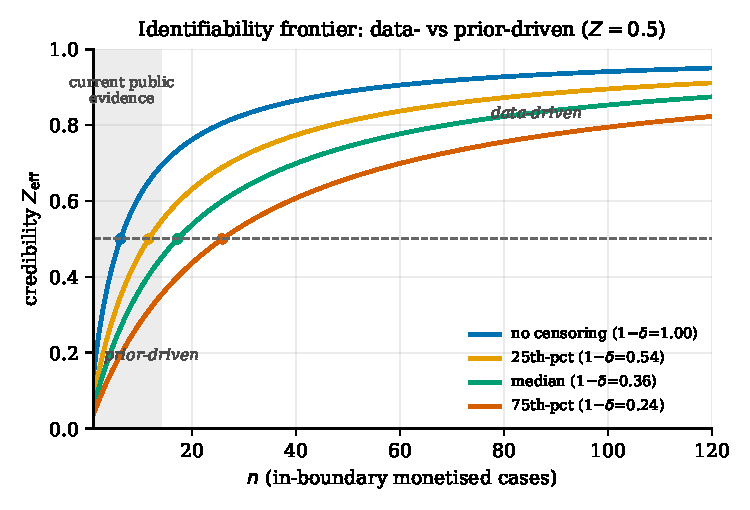
\includegraphics[width=0.70\textwidth]{fig_frontier.pdf}
\caption{The identifiability frontier. Credibility $Z_{\mathrm{eff}}$ versus in-boundary sample
size $n$ for several disclosure-censoring levels ($k=\sigma^2/\tau^2=6.25$). The $Z=\tfrac12$ line
separates the prior-driven and data-driven regimes; markers show $n^\star=k/(1-\delta)$. Heavier
censoring pushes $n^\star$ outward; currently available public in-boundary evidence (shaded) sits
in the prior-driven region.}
\label{fig:frontier}
\end{figure}

\begin{proposition}[Layer-pricing implication; location only]\label{prop:lev}
For a lognormal severity the limited expected value of a layer attaching at $A$ with limit $L$
follows the standard closed form \citep{klugman2019}; substituting the credibility location
$\mu_{\text{post}}=m_0+Z_{\text{eff}}(\hat\theta-m_0)$ and predictive variance
$\sigma_{\text{pred}}^2=\sigma^2+\tau^2(1-Z_{\text{eff}})$ shows the layer premium is updated by
data only through the \emph{location}. Because $\sigma$ (hence the tail) is held at the proxy,
upper excess layers ($A\gg e^{m_0}$) are insensitive to data \emph{by construction}, not as a
consequence of the frontier; only working layers near $e^{\mu_{\text{post}}}$ respond to data.
\end{proposition}
\noindent Proposition~\ref{prop:lev} is therefore a caution, not a pricing tool for excess
layers: a credible excess-layer treatment requires updating the tail, which we do not do here.

\paragraph{Sensitivity of the frontier.} Table~\ref{tab:val} tabulates $n^\star=k/(1-\delta)$.
The frontier moves by $2$--$4\times$ with censoring and by the same order with prior strength
$k$; it is not a single number.
\begin{table}[h]\centering
\begin{tabular}{l|c|cccc}
\toprule
& & \multicolumn{4}{c}{\textbf{Required } $n^\star$ \textbf{ by prior strength } $k=\sigma^2/\tau^2$}\\
\textbf{Censoring} & $1-\delta(\alpha)$ & Strong ($k{=}10$) & Baseline ($k{=}6.25$) & Weak ($k{=}4$) & Diffuse ($k{=}2$)\\
\midrule
none & 1.000 & 10.0 & 6.2  & 4.0 & 2.0\\
25th pct & 0.535 & 18.7 & 11.7 & 7.5 & 3.7\\
median & 0.363 & 27.5 & 17.2 & 11.0& 5.5\\
75th pct & 0.242 & 41.3 & 25.8 & 16.5& 8.3\\
\bottomrule
\end{tabular}
\caption{Frontier $n^\star$ across censoring and (weakly identified) prior strength $k$. Both
axes are assumptions, not estimates; the regime verdict depends on the cell chosen.}
\label{tab:val}
\end{table}

\section{Proxy-line priors}\label{sec:priors}
We illustrate prior calibration from published cyber/operational-risk severity statistics
(Table~\ref{tab:priors}), matching a lognormal by $\mu=\log(\text{median})$,
$\sigma=\sqrt{2(\log\text{mean}-\log\text{median})}$. \emph{This moment-match is unreliable when
the proxy is heavy/infinite-mean tailed} \citep{elingjung2022,cremer2023}; we use it only to
locate a plausible $k$, not as a tail model, and note the unresolved tension between a lognormal
location model and the heavy tails the proxy exhibits.

\begin{table}[h]\centering
\begin{tabular}{lccc}
\toprule
proxy sub-line & median (\$M) & mean (\$M) & source\\
\midrule
Privacy: unauthorized disclosure & 2.92 & 9.49  & \citet{malavasi2021}\\
Data: malicious breach           & 0.94 & 28.96 & \citet{malavasi2021}\\
Identity: fraudulent use         & 0.16 & 1.83  & \citet{malavasi2021}\\
Cyber aggregate                  & 0.11 & 16.84 & \citet{cremer2023}\\
Financial op-risk ($>\$100$k)    & 1.10 & 24.95 & \citet{elingjung2022}\\
\bottomrule
\end{tabular}
\caption{Published proxy severity statistics (different units of observation; pooling is itself
an approximation). The \$100k floor is a disclosure threshold, motivating Section~\ref{sec:trunc}.}
\label{tab:priors}
\end{table}

\section{Illustrative empirical localisation}\label{sec:empirical}
\paragraph{Screen.} We re-screen \emph{all} $1{,}505$ AIID incidents (CC-BY-SA~4.0) against the
Section~\ref{sec:model} inclusion boundary---not only those matching a monetary regex, which
miss small or foreign-currency figures (e.g.\ the canonical \emph{Moffatt v.\ Air Canada}
chatbot case). Out-of-boundary classes (wrongful-arrest, biometric/BIPA, physical-safety,
employment, government-benefit) are excluded with documented per-case reasons; the screen is
released as auditable code and CSV.

\paragraph{The in-boundary count is small and heterogeneous, and that is the finding.} The
re-screen returns $181$ in-boundary candidates. Categorising them is decisive: $75$ are
copyright/IP matters carrying \emph{unpaid} demands (multi-billion-dollar prayers for relief in
training-data suits), $35$ are regulatory fines, $16$ are lawyer-sanction matters (AI-fabricated
citations), and only $\sim$$28$ are genuine ``AI service $\to$ third-party economic loss''. Of
those, the cases with a confirmed \emph{paid} figure number only a handful and span four orders
of magnitude---from the Air Canada chatbot tribunal award ($\approx$CAD\$812) to AI-defamation
settlements of \$5M (Meta) and \$15M (Google)---and are dominated by defamation rather than the
advisory/decision-support losses the boundary targets. Pooling the headline figures of distinct
legal regimes (copyright demands, fines, sanctions, settlements), as a naive screen does, both
mis-classifies and wildly overstates the severity sample (Figures~\ref{fig:funnel}--\ref{fig:severity}).

\begin{figure}[h]\centering
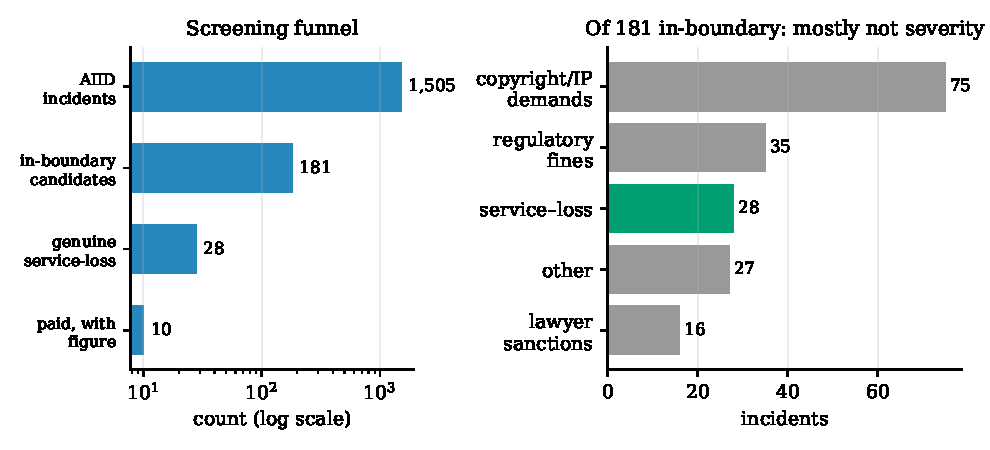
\includegraphics[width=0.92\textwidth]{fig_funnel.pdf}
\caption{Screening funnel (left) and category composition of the $181$ in-boundary candidates
(right). The overwhelming majority are copyright/IP demands, regulatory fines, or lawyer-sanction
matters; only $\sim$$28$ are genuine ``AI service $\to$ third-party economic loss'', and fewer
still carry a paid figure---the sparsity that is the empirical finding.}
\label{fig:funnel}
\end{figure}

\begin{figure}[h]\centering
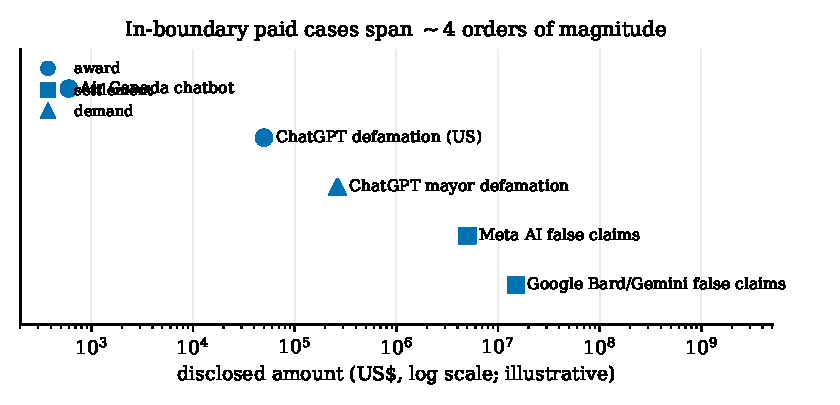
\includegraphics[width=0.80\textwidth]{fig_severity.pdf}
\caption{Illustrative in-boundary paid cases on a log-dollar scale (amounts approximate, pending
primary-source verification). The span of roughly four orders of magnitude---and the dominance of
defamation---illustrates why a severity distribution cannot be calibrated from this sample.}
\label{fig:severity}
\end{figure}

\paragraph{This is not a verified severity dataset, and we do not treat it as one.} Even the
in-boundary screen has material defects, each of which alone undermines a pricing inference:
(a)~figures are secondary, mixed-currency, nominal across $\sim$2015--2025 and not yet confirmed
against court/regulator primary sources; (b)~loss types (settlement / award / fine / demand) are
not commensurable and must not be pooled; (c)~the sample is \emph{right}-censored by policy
limits and ability-to-pay (settlements cluster at tower limits, not true harm), compressing
$\hat\sigma$, and this is unmodelled; (d)~the disclosure mechanism is selection-on-unobservables
(large losses settle under NDA \emph{to avoid} disclosure), violating the fixed-threshold
left-truncation the model assumes; (e)~recent cases are immature (IBNR); (f)~AIID is itself
curated for notable incidents---a second selection layer away from an underwriter's exposure
population.

\paragraph{What can be said.} With only a handful of genuinely in-boundary paid settlements, the
severity \emph{location} cannot be estimated with any precision, let alone localised on the
frontier of Table~\ref{tab:val}: any $Z_{\text{eff}}$ computed from such an $n$ is dominated by
sampling and classification noise far exceeding the $14$-versus-$17$ margins previously claimed,
and the verdict flips across plausible prior strengths $k$ (which is itself weakly identified).
\textbf{The prior-driven-versus-data-driven regime is therefore not identified from current
public data.} That negative result---public AI-liability loss experience is too sparse,
heterogeneous, and selection-distorted to displace a proxy prior---is the paper's defensible
empirical message. A severity \emph{calibration} would require non-public insurer claims data;
public catalogues can support a screen and an identifiability statement, not a rate.

\section{Limitations and threats to validity}
(i)~\textbf{Frequency} is non-identifiable from public data (a result, not an omission).
(ii)~\textbf{Location only}: the result updates $\theta$, not the tail $\sigma$; the loss cost is
tail-driven, so excess-layer pricing is out of scope (Proposition~\ref{prop:lev}).
(iii)~\textbf{Independence}: the model assumes i.i.d.\ severities, but AI failures are
correlated/fleet-wide (one model defect $\to$ many simultaneous claims), an accumulation risk
the i.i.d.\ credibility machinery and the idiosyncratic cyber proxy both ignore.
(iv)~\textbf{Proxy isomorphism} is assumed, not defended: cyber severity scales with records
breached, AI economic loss with downstream reliance on wrong outputs---different tail drivers.
(v)~\textbf{Heavy tails}: the lognormal location model contradicts the heavy/infinite-mean cyber
tails cited; moment-matching $\sigma$ is unreliable there.
(vi)~\textbf{Data}: right-censoring, selection-on-unobservables, IBNR immaturity, currency/year
mixing, and boundary violations (above) make the empirical set illustrative only.
(vii)~\textbf{Scope of ``agent''}: the AIID-era cases are pre-agentic (advisory/content tools),
so claims about autonomous AI \emph{agents} are not supported by this sample.
(viii)~\textbf{Truncation bias}: $\bar Y\mid Y>t$ overstates $\theta$; a Heckman/Tobit correction
is deferred.

\section{Conclusion}
Framing emerging-risk severity as an identifiability question---and giving an explicit,
censoring-inflated frontier $n^\star(t)$---is a clean applied lens, and the honest empirical
finding is a \emph{negative} one: with current public data the prior-/data-driven regime for
AI-liability severity is not identified. The mathematical components are standard recombinations,
not new theorems; the contribution is the lens and its candid localisation. Realistic venue is an
applied actuarial outlet (e.g.\ \emph{Variance} or \emph{Risks}). Future work that would make this
a substantive contribution: a sourced, in-boundary, censoring- and selection-corrected dataset; an
accumulation/dependence model for fleet-correlated AI failures; and extension of the credibility
update from the location to the tail and the loss-cost functional.

\paragraph{Reproducibility.} Code, proxy priors, the truncation validation, and the screening
protocol are at \url{https://github.com/tayyub-ai/actuarial-loss-cost-modelling-for-ai-agent-liability}.
The illustrative case set is \emph{not} a verified dataset and is labelled as such.

\bibliographystyle{plainnat}
\begin{thebibliography}{99}
\bibitem[Biener et al.(2015)]{biener2015cyber} Biener, C., Eling, M., Wirfs, J. H. (2015). Insurability of cyber risk: An empirical analysis. \emph{Geneva Papers on Risk and Insurance} 40(1), 131--158.
\bibitem[B\"uhlmann \& Gisler(2005)]{buhlmann2005} B\"uhlmann, H., Gisler, A. (2005). \emph{A Course in Credibility Theory and its Applications}. Springer.
\bibitem[Chen(2026)]{chen2026} Chen, H.-H. (2026). Insuring Every Action: An Authority Frontier Framework for Runtime Actuarial Control of Autonomous AI Systems. arXiv:2605.25632.
\bibitem[Clark(2002)]{clark2002cat} Clark, K. M. (2002). The use of computer modeling in estimating and managing future catastrophe losses. \emph{Geneva Papers on Risk and Insurance} 27(2), 181--195.
\bibitem[Cremer et al.(2023)]{cremer2023} Cremer, F., et al. (2023). The nature of losses from cyber-related events. \emph{Journal of Cybersecurity} 9(1), tyac016.
\bibitem[Diaconis \& Ylvisaker(1979)]{diaconis1979} Diaconis, P., Ylvisaker, D. (1979). Conjugate priors for exponential families. \emph{Annals of Statistics} 7(2), 269--281.
\bibitem[Eling \& Jung(2022)]{elingjung2022} Eling, M., Jung, K. (2022). Heterogeneity in cyber loss severity. \emph{Risk Management} 24, 273--297.
\bibitem[Farkas et al.(2021)]{farkas2021} Farkas, S., Lopez, O., Thomas, M. (2021). Cyber claim analysis using generalized Pareto regression trees. \emph{Insurance: Mathematics and Economics} 98, 92--105.
\bibitem[G\'omez-D\'eniz \& V\'azquez-Polo(2022)]{gomezdeniz2022} G\'omez-D\'eniz, E., V\'azquez-Polo, F. (2022). Exact credibility reference Bayesian premiums. \emph{Insurance: Mathematics and Economics} 105, 128--143.
\bibitem[Han et al.(2022)]{han2022} Han, Z., Ye, K., Wang, M. (2022). On the normalized power prior. \emph{Computational Statistics \& Data Analysis}. arXiv:2204.05615.
\bibitem[Hobbs et al.(2011)]{hobbs2011} Hobbs, B., Carlin, B., Mandrekar, S., Sargent, D. (2011). Hierarchical commensurate and power prior models. \emph{Biometrics} 67(3), 1047--1056.
\bibitem[Ibrahim \& Chen(2000)]{ibrahim2000} Ibrahim, J., Chen, M.-H. (2000). Power prior distributions for regression models. \emph{Statistical Science} 15(1), 46--60.
\bibitem[Jewell(1974)]{jewell1974} Jewell, W. (1974). Credible means are exact Bayesian for exponential families. \emph{ASTIN Bulletin} 8(1), 77--90.
\bibitem[Kim \& Jeon(2013)]{kimjeon2013} Kim, J.H.T., Jeon, Y. (2013). Credibility theory based on trimming. \emph{Insurance: Mathematics and Economics} 53(1), 36--47.
\bibitem[Klugman et al.(2019)]{klugman2019} Klugman, S., Panjer, H., Willmot, G. (2019). \emph{Loss Models: From Data to Decisions}, 5th ed. Wiley.
\bibitem[Leung et al.(2026a)]{leung2026insurability} Leung, A., Zhang, R., Ling, E., Toyoda, K., Loh, S.M. (2026). The Insurability Frontier of AI Risk. arXiv:2605.18784.
\bibitem[Leung et al.(2026b)]{leung2026cer} Leung, A., Zhang, R., Toyoda, K., Loh, S.M. (2026). From Control Boundary to Insurance Claim: the CER Framework. arXiv:2606.03777.
\bibitem[Malavasi et al.(2021)]{malavasi2021} Malavasi, M., et al. (2021). Cyber risk frequency, severity and insurance viability. arXiv:2111.03366.
\bibitem[Schmidli et al.(2014)]{schmidli2014} Schmidli, H., et al. (2014). Robust meta-analytic-predictive priors. \emph{Biometrics} 70(4), 1023--1032.
\bibitem[Zhu(2026)]{zhu2026} Zhu, Q. (2026). Insurance of Agentic AI. arXiv:2606.05449.
\end{thebibliography}
\end{document}
